\section{Results}
\suppressfloats[t]

\subsection{Primary Held-Out Performance}


EVO-F has the lowest mean excess among LLM strategies, but no discovered
method outperforms GR+P on average (Table~\ref{tab:primary}).
The primary EVO-F--IND contrast is $-0.148$ percentage points
(original run-index-paired 95\% CI: $[-0.699,0.220]$).
The secondary EVO-F--EVO-P contrast is $-0.305$ points
($[-1.004,0.174]$); EVO-P--IND is $+0.157$
($[-0.659,1.026]$). These intervals establish neither a reliable advantage
nor equivalence.

\begin{samepage}
Independent method-run resampling gives intervals of $[-0.890,0.512]$
for EVO-F--IND and $[-1.049,0.314]$ for EVO-F--EVO-P
(Figure~\ref{fig:transfer}), leaving the interpretation unchanged. Greedy is already optimal on 40 of 60 graphs.
On the remaining 20, EVO-F closes no mean headroom ($-0.25\%$ of the
available gap). Limited headroom therefore constrains, but does not fully
explain, the lack of improvement.\par
\end{samepage}

\begin{figure}[!htbp]
\centering
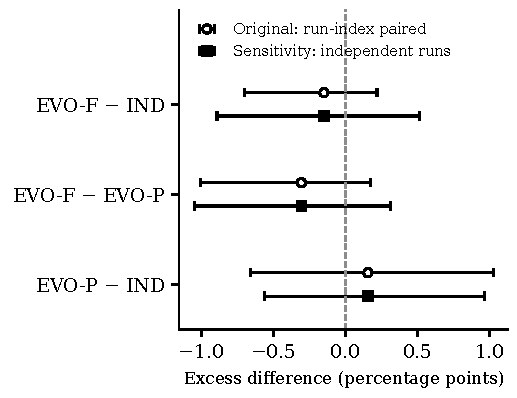
\includegraphics[width=\columnwidth]{figures/primary_bootstrap_sensitivity.pdf}
\caption{Primary and secondary contrasts under the original run-index-paired
bootstrap and the independent-run sensitivity. Both use paired graph indices,
five runs per strategy and 5,000 draws. Negative values favor the first
method; all intervals contain zero.}
\label{fig:transfer}
\end{figure}

\subsection{Synthetic Distribution Shifts}
\begin{table}[!htbp]
\centering\small
\setlength{\tabcolsep}{3pt}
\caption{Mean excess cost (\%) on synthetic shifts, each with 60 graphs.
Hub-cost variants share the primary topologies and cost multisets.
Size80 changes graph size; BA changes topology. Primary ID/random values
are in Table~\ref{tab:primary}. Negative values favor the method.}
\label{tab:shift}
\begin{tabular*}{\columnwidth}{@{\extracolsep{\fill}}lrrrr@{}}
\toprule
Method & Hub-exp. & Hub-cheap & Size80 & BA\\
\midrule
% Generated from saved JSON by scripts/reproduce_results.py.
IND & -0.378 & +0.302 & +0.213 & +0.065 \\
EVO-P & -0.579 & +0.548 & +0.294 & +1.322 \\
EVO-F & -0.615 & +0.093 & +0.168 & +1.438 \\
RS-PARAM & +0.827 & +0.129 & +0.401 & -0.349 \\
GR+P & +0.000 & +0.000 & +0.000 & +0.000 \\
RGR+P & -1.017 & +0.088 & -0.472 & -0.483 \\
Reverse-delete & +0.722 & +1.547 & +1.150 & +13.048 \\
\bottomrule

\end{tabular*}
\end{table}

Controlled cost--degree alignment changes performance
(Table~\ref{tab:shift}). All LLM strategies improve on greedy on average with
hub-expensive costs, yet the handcrafted RGR+P rule improves more.
Because topology and the cost multiset are fixed, this comparison concerns
cost allocation rather than cost scale.

On size and topology shifts, the LLM strategies lose to greedy on average.
RGR+P improves in both, while RS-PARAM improves only on BA. A useful
priority exists within the scaffold but is not consistently recovered by
evolution. Section~\ref{sec:rarity_form} analyzes its rarity weighting.

\subsection{Published T1/T2 Transfer}
\begin{table}[!htbp]
\centering\small
\setlength{\tabcolsep}{3pt}
\caption{External transfer: mean excess (\%) and median first-call runtime
(seconds, T1/T2). Each family has 24 weighted instances on shared topologies;
search methods use all five frozen winners. Timing describes the reference
interpreter. Full outcome counts and medians remain in the repository.}
\label{tab:external}
\begin{tabular*}{\columnwidth}{@{\extracolsep{\fill}}lrrr@{}}
\toprule
Method & T1 excess & T2 excess & \shortstack{Time\\T1/T2 (s)}\\
\midrule
% Generated from saved JSON by scripts/reproduce_results.py.
GR+P & +0.00 & +0.00 & 0.992/1.039 \\
RGR+P & -1.26 & -0.58 & 3.756/1.768 \\
Reverse-delete & +6.55 & +1.82 & 0.013/0.008 \\
IND & +0.18 & -0.08 & 4.011/2.881 \\
EVO-P & +0.20 & -0.03 & 4.104/2.954 \\
EVO-F & +0.40 & +0.16 & 3.842/2.628 \\
RS-PARAM & +1.60 & +0.80 & 8.377/5.257 \\
\bottomrule

\end{tabular*}
\end{table}

Frozen programs transfer without benchmark-specific tuning.
EVO-F has higher mean excess than IND and EVO-P in both weight families,
while RGR+P has the lowest (Table~\ref{tab:external}).
IND and EVO-P improve slightly on greedy under degree-dependent T2
weights; EVO-F does not. External family averages therefore show no
descriptive feedback advantage. Size/density rankings are mixed.

\begin{samepage}
RGR+P's gains are uneven: its wins/ties/losses against greedy are
11/11/2 on T1 and 7/15/2 on T2.\par
\end{samepage}

\begin{samepage}
All external solutions pass independent feasibility checks. CP-SAT certifies
only five T2 instances, all at $n=100$, and no T1 instance within its search
limit; exact-gap statistics on those five cases are not representative
of either full family.\par
\end{samepage}

\subsection{Classical Solver at 50 ms}
\begin{table}[!htbp]
\centering\small
\setlength{\tabcolsep}{3pt}
\caption{Same-session primary-graph control under a 50 ms end-to-end target.
Fixed methods have 180 measured calls and EVO-F 900. Late counts calls
exceeding the target; gaps and hits use certified optima.}
\label{tab:control}
\begin{tabular}{lrrrr}
\toprule
Method & Gap (\%) & Hits (\%) & Median ms & Late\\
\midrule
% Generated from saved JSON by scripts/reproduce_results.py.
GR+P & 2.89 & 66.7 & 4.17 & 0/180 \\
RGR+P & 3.37 & 63.3 & 10.50 & 0/180 \\
EVO-F & 3.21 & 63.3 & 14.94 & 0/900 \\
CP-SAT50 & 0.00 & 100.0 & 7.39 & 0/180 \\
\bottomrule

\end{tabular}
\end{table}

CP-SAT50 reaches every primary optimum in every repeat, with median
latency 7.39 ms versus 14.94 ms for EVO-F and no deadline overrun
(Table~\ref{tab:control}). On these original $n=40$ graphs, it offers both
better solution quality and lower median latency for the evaluated reference
implementation. This comparison concerns neither every possible optimized
learned heuristic nor the external benchmark's longer certification attempts.

Discovery used 800 attempts, yielding 513 novel-valid proposals within runs
and 287 invalid or duplicate proposals. The 600 LLM attempts cost
US\$0.0806 (IND), US\$0.1115 (EVO-P), and US\$0.1834 (EVO-F),
including unsuccessful and duplicate proposals. Recorded training solver
time was 58.2, 145.9, and 105.2 seconds, respectively; RS-PARAM used
323.6 seconds and no API calls. These totals include seed evaluations
but exclude reference setup, parsing, search overhead, and API waiting;
full evaluator wall time was not recorded. Discovery resources are
separate from the deployment runtimes above, which measure execution
of frozen heuristics.
